\documentclass[12pt,a4paper]{article}

\usepackage[utf8]{inputenc}
\usepackage[T2A]{fontenc}
\usepackage[russian]{babel}
\usepackage{amsmath, amssymb, amsthm, amsfonts}
\usepackage{graphicx}
\usepackage{hyperref}
\usepackage[margin=2cm]{geometry}
\usepackage{cite}
\usepackage{setspace}
\usepackage{float}
\usepackage{booktabs}
\usepackage{caption}
\usepackage{subcaption}

\onehalfspacing

\hypersetup{
    pdftitle={Исследование влияния вида задачи для уравнения гармонического осциллятора на решение PINN},
    pdfauthor={Донецков А.Д., Бакакин В.Д., Жулев Е.М.},
    pdfsubject={Отчёт},
    pdfkeywords={PINN, ОДУ, гармонический осциллятор, машинное обучение}
}

\title{Исследование влияния вида задачи для уравнения гармонического осциллятора на решение PINN}
\author{
Донецков А.Д.\thanks{E-mail: andrey.donetskov@gmail.com}, 
Бакакин В.Д., 
Жулев Е.М. \\
\textit{НИЯУ МИФИ}
}
\date{\today}

\begin{document}

\maketitle

\begin{abstract}
В данном отчёте рассматривается применение метода физически -- информированных нейронных сетей \textbf{PINN} (Physics-Informed Neural Networks) для решения уравнения гармонического осциллятора с вынуждающей силой. Исследуется влияние различных формулировок задачи Коши на точность и сходимость метода PINN. Представлены сравнительные результаты, демонстрирующие различия в скорости сходимости, устойчивости обучения и точности. Дополнительно проведён анализ устойчивости методов и их применимость к системам с резонансом.
\end{abstract}

\tableofcontents
\newpage

\section{Введение}
Одной из важных задач в области вычислительной физики и механики является решение уравнений движения гармонического осциллятора. Классический гармонический осциллятор описывается различными дифференциальными уравнениями как второго, так и первого порядка. В последнее десятилетие активно развиваются нейросетевые методы решения дифференциальных уравнений, в частности метод физически-информированных нейронных сетей (PINN) \cite{Lagaris1998,Raissi2019}.

Метод PINN позволяет интегрировать физические законы непосредственно в процесс обучения нейронной сети, что обеспечивает получение решений, согласующихся с заданными дифференциальными уравнениями и граничными условиями. Однако эффективность метода может зависеть от выбора формулировки задачи Коши.

Цель данного исследования --- сравнить влияние различных формулировок задачи Коши для уравнения гармонического осциллятора на точность и эффективность метода PINN.

\section{Постановка задачи}
Рассматриваются три различных формулировки задачи Коши для уравнения гармонического осциллятора с вынуждающей силой, по два набора параметров для каждой --- для случаев резонанса и его отсутствия:

\subsection{ОДУ второго порядка}
Уравнение вида
\begin{equation}
\begin{cases}
\dfrac{d^2x}{dt^2} + \omega_0^2 x = -A\cos(\omega t), \\
x(0) = x_0, \\
\dfrac{dx}{dt}(0) = v_0.
\end{cases}
\end{equation}
непосредственно описывает динамику гармонического осциллятора.

\textbf{Применение:}
\begin{itemize}
    \item \textbf{Физика колебаний:} Моделирование механических систем, таких как пружинные маятники или электрические колебательные контуры, где присутствуют гармонические колебания.
    \item \textbf{Анализ устойчивости:} Исследование устойчивости систем, подверженных периодическим внешним воздействиям.
\end{itemize}

\subsection{Системы ОДУ первого порядка}
\subsubsection{Система (2)}
\begin{equation}
\begin{cases}
\dfrac{dx}{dt} = y, \\
\dfrac{dy}{dt} = -\omega_0^2 x - A\cos(\omega t), \\
x(0) = x_0, \\
y(0) = v_0.
\end{cases}
\end{equation}

\subsubsection{Система (3)}
\begin{equation}
\begin{cases}
\dfrac{dx}{dt} = \omega_0 y - \dfrac{A}{\omega}\sin(\omega t), \\
\dfrac{dy}{dt} = -\omega_0 x, \\
x(0) = x_0, \\
y(0) = \dfrac{v_0}{\omega_0}.
\end{cases}
\end{equation}

\textbf{Применение:}
\begin{itemize}
    \item \textbf{Численные методы:} Многие численные алгоритмы, такие как методы Рунге -- Кутты, разработаны для систем первого порядка, что делает эту форму удобной для компьютерного моделирования.
    \item \textbf{Сложные системы:} Анализ систем с несколькими степенями свободы, где каждая степень описывается своим уравнением первого порядка.
\end{itemize}

\textbf{Примечание:}
Разные системы дифференциальных уравнений первого порядка могут быть полезны в случаях, когда форма упрощает аналитическое или численное решение, в зависимости от характера внешней силы или других факторов.

\section{Ключевые особенности PINN}

\begin{minipage}[t]{0.45\textwidth}
    \small
    \textbf{Преимущества PINN:}
    \begin{itemize}
        \item Интеграция физических законов в процесс обучения для получения физически корректных решений.
        \item Использование автоматического дифференцирования для эффективного вычисления градиентов сложных выражений.
        \item Применимость к различным задачам, включая ОДУ, УЧП и их системы.
    \end{itemize}
\end{minipage}
\hfill
\vrule width 0.5pt
\hfill
\begin{minipage}[t]{0.45\textwidth}
    \small
    \textbf{Ограничения PINN:}
    \begin{itemize}
        \item Трудности с аппроксимацией разрывных функций.
        \item Низкая эффективность при решении жестких и хаотических систем ОДУ.
        \item Застревание в локальных оптимумах.
        \item Сложности в балансировке различных компонентов функции потерь.
    \end{itemize}
\end{minipage}

\section{Методология}

\subsection{Архитектура нейронной сети}
\begin{itemize}
    \item \textbf{Входной слой:} 1 нейрон (время $t$).
    \item \textbf{Скрытые слои:} 5 слоёв по 20 нейронов каждый с функцией активации $\sin$.
    \item \textbf{Выходной слой:} 1 или 2 нейрона (в зависимости от системы ОДУ).
\end{itemize}

\subsection{Функционал потерь}
Функционал потерь определяется как
\[
loss = loss_{interior} + \lambda_{bc} \cdot loss_{boundary},
\]
где:
\begin{enumerate}
    \item $loss_{interior}$ --- потери на уравнении (MSE по residual), учитывающие форму дифференциального уравнения.
    \item $loss_{boundary}$ --- потери на граничных условиях (MSE между предсказанием и истинным значением).
\end{enumerate}
Весовой коэффициент ограничения ($\lambda_{bc}$) выбран равным 50.

\subsection{Процесс обучения}
Обучение модели проводилось с использованием оптимизатора Adam с шагом обучения $10^{-3}$ для минимизации функции потерь. Этот оптимизатор показал наилучшие результаты в предварительных экспериментах. Функцией активации был выбран синус.

\subsection{Параметры эксперимента}
\begin{itemize}
    \item \textbf{Интервал обучения:} $[-5, 15]$.
    \item \textbf{Шаг разбиения:} $0.05$.
    \item \textbf{Количество запусков:} 5 для каждой системы и каждого случая (с резонансом и без него).
    \item \textbf{Метрика оценки:} \textbf{MAE} (mean absolute error).
\end{itemize}

\section{Результаты}

Для каждой системы было произведено пять запусков обучения, как для случая с резонансом, так и без него. Результаты представлены ниже.

\subsection{Система ОДУ второго порядка (1)}

\begin{figure}[H]
    \centering
    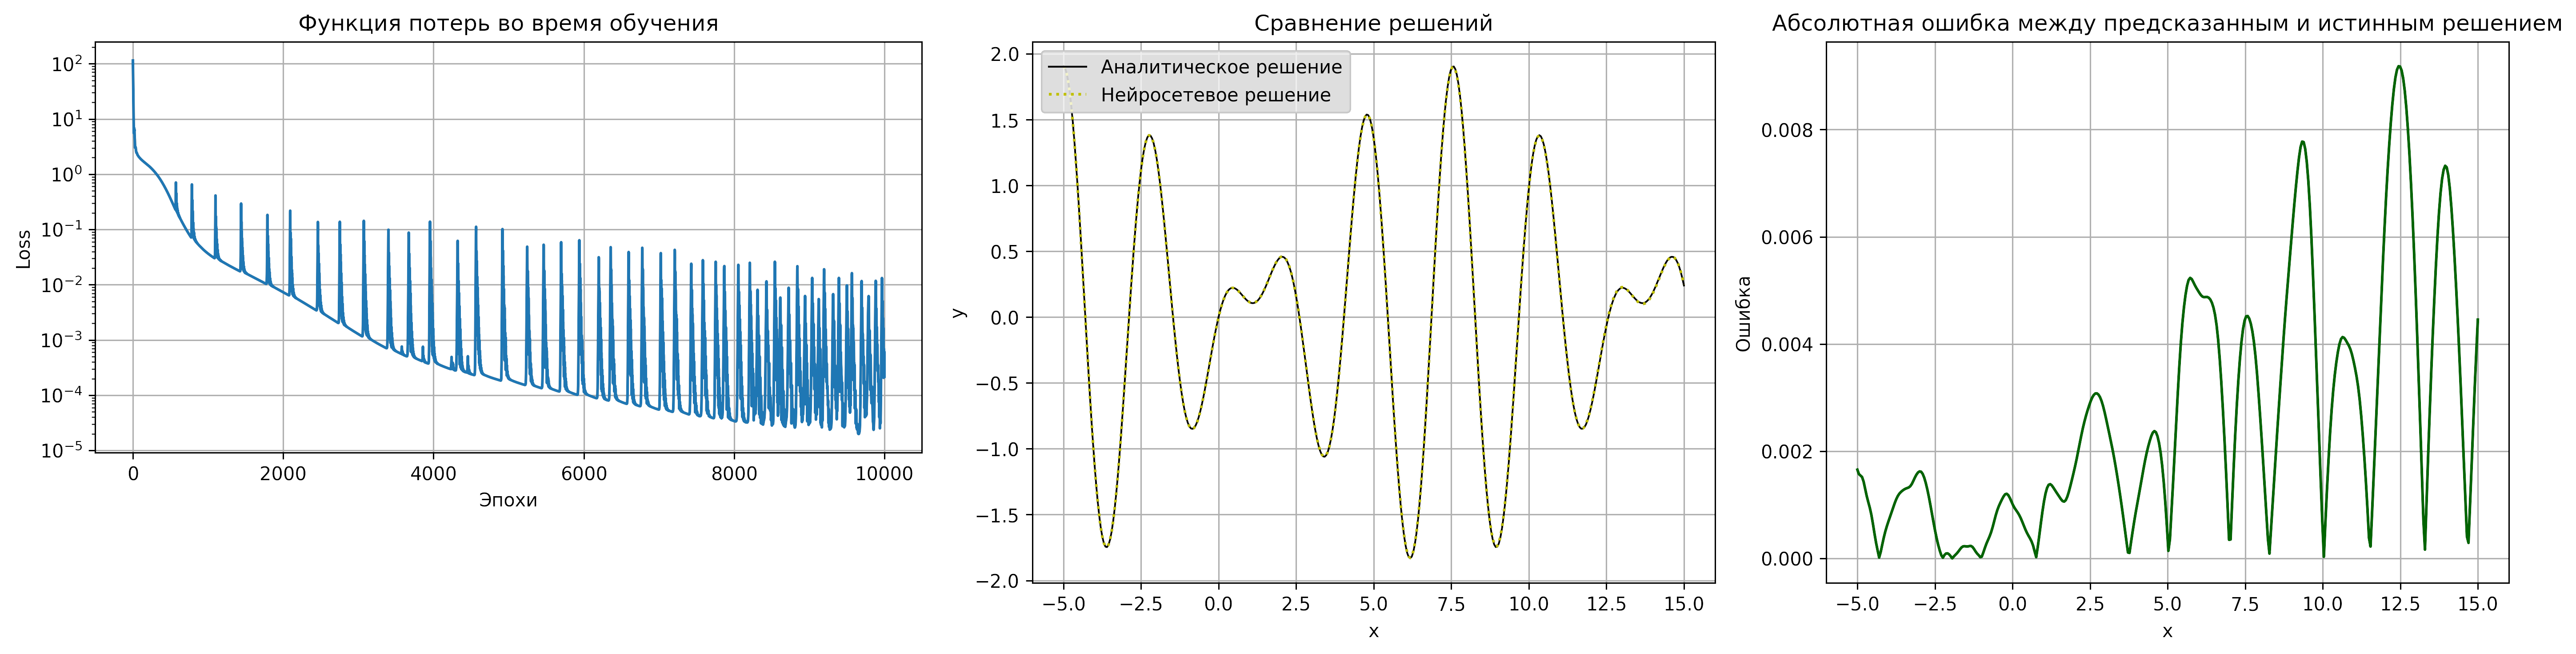
\includegraphics[width=0.8\textwidth]{images/Loss&x_ODE_of_the_second_order.png}
    \caption{Функция потерь для ОДУ второго порядка}
    \label{fig:loss_second_order}
\end{figure}

\begin{figure}[H]
    \centering
    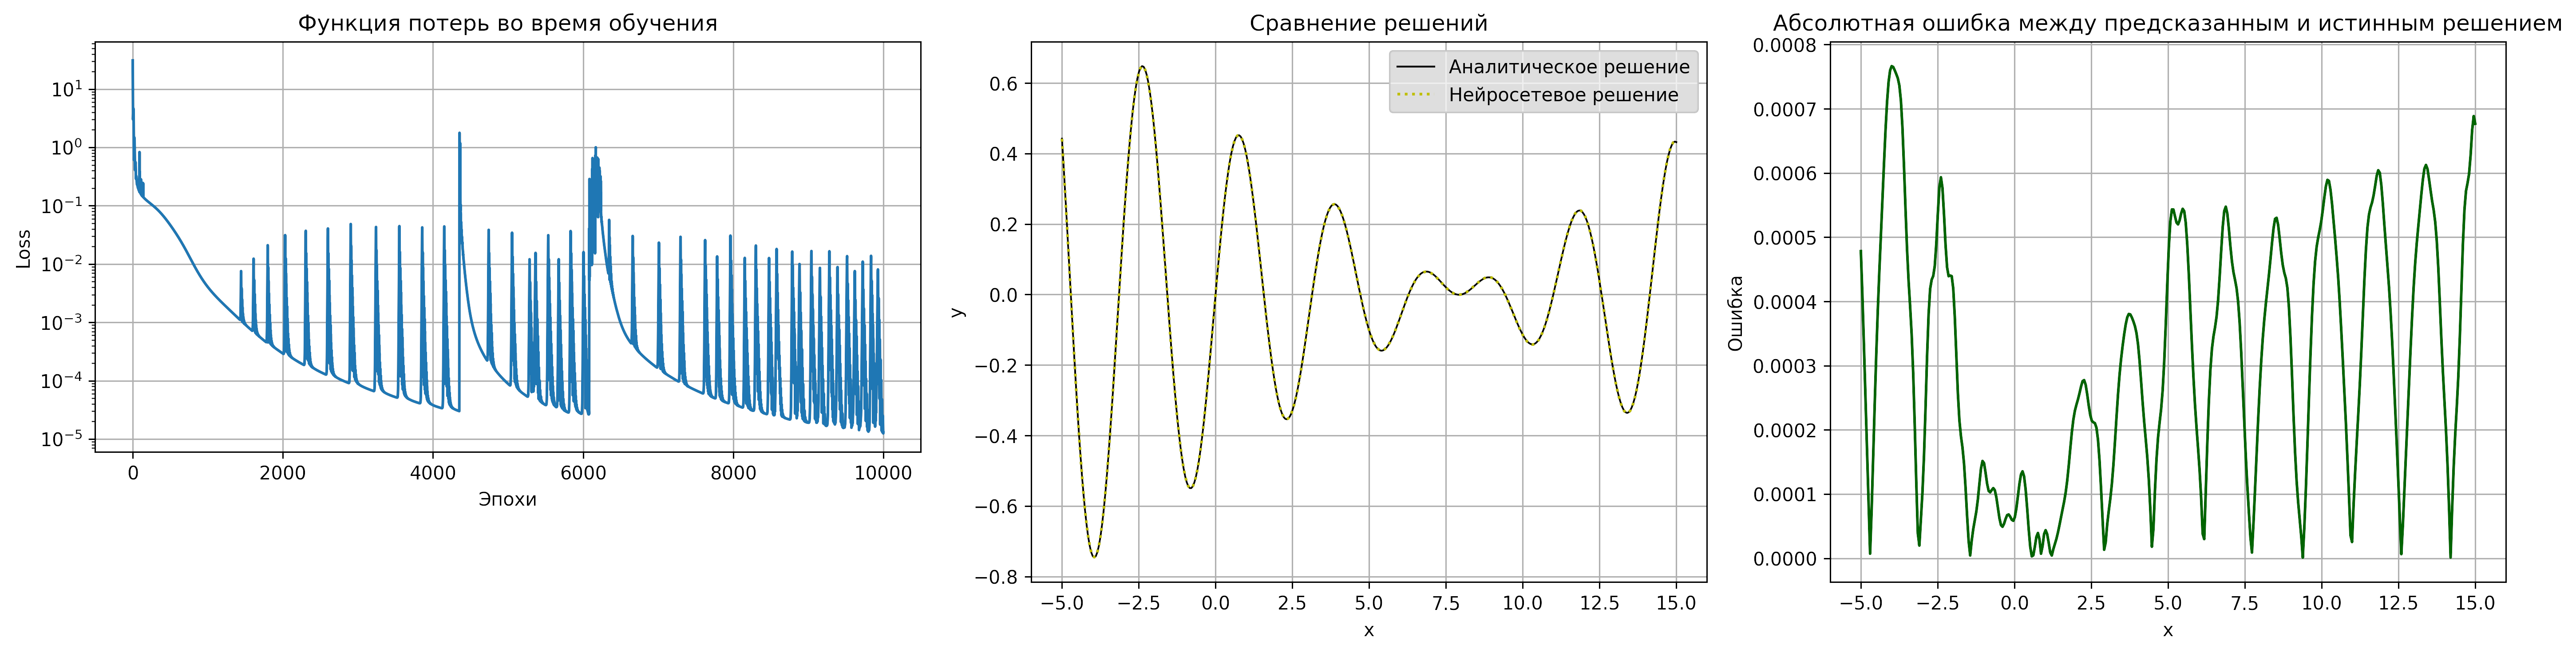
\includegraphics[width=0.8\textwidth]{images/Loss&x_ODE_of_the_second_order_resonance.png}
    \caption{Функция потерь для ОДУ второго порядка с резонансом}
    \label{fig:loss_second_order_resonance}
\end{figure}

\begin{table}[h!]
    \centering
    \begin{tabular}{|c|c|c|c|}
    \hline
    \multicolumn{2}{|c|}{\textbf{Без резонанса}} & \multicolumn{2}{|c|}{\textbf{С резонансом}} \\
    \hline
    \textbf{MAE $x, 10^{-2}$} & \textbf{MAE $\dfrac{dx}{dt}, 10^{-2}$} & \textbf{MAE $x, 10^{-2}$} & \textbf{MAE $\dfrac{dx}{dt}, 10^{-2}$} \\
    \hline
    1.1879 & 2.4357 & 1.1877 & 2.4116 \\
    1.2033 & 2.4247 & 1.2502 & 2.5555 \\
    1.6343 & 3.0803 & 1.4000 & 2.8247 \\
    1.2127 & 2.4514 & 1.2128 & 2.4863 \\
    1.1406 & 2.3287 & 1.2032 & 2.3616 \\
    \hline
    \textbf{1.2758} & \textbf{2.5442} & \textbf{1.2508} & \textbf{2.5279} \\
    \hline
    \end{tabular}
    \caption{ОДУ второго порядка}
\end{table}

\begin{itemize}
    \item Высокая точность и быстрая сходимость.
    \item Возможные проблемы с локальными минимумами.
\end{itemize}

\newpage

\subsection{Система ОДУ первого порядка (2)}

\begin{figure}[H]
    \centering
    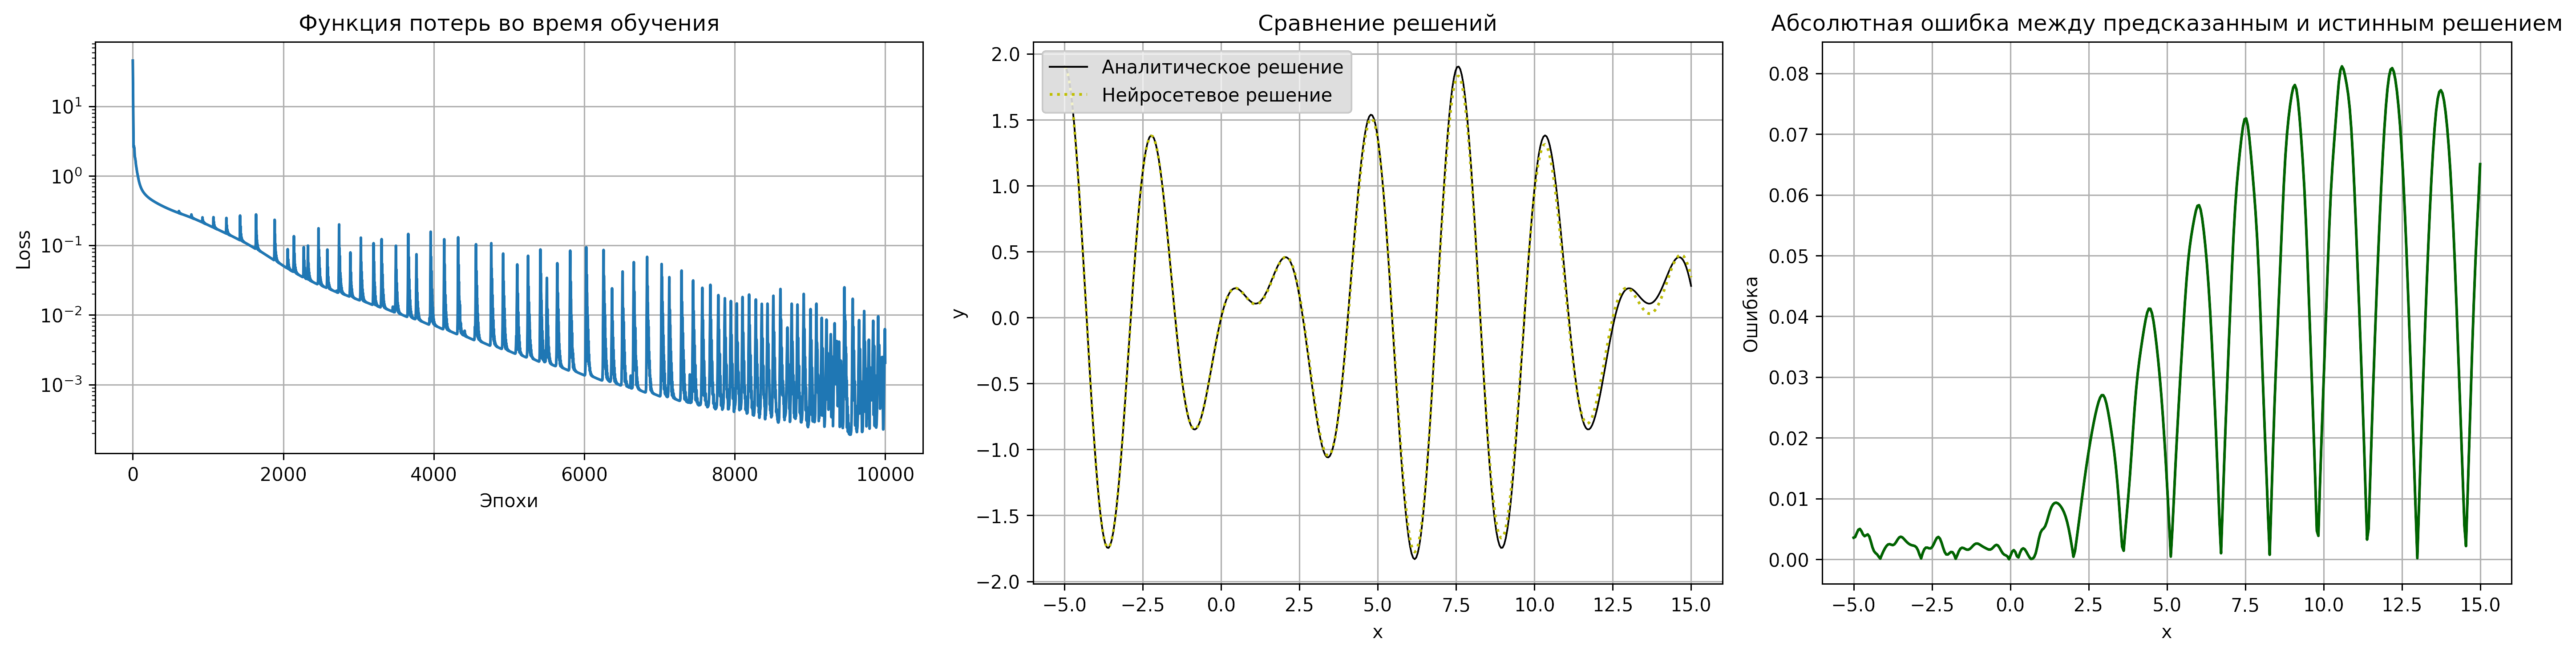
\includegraphics[width=0.8\textwidth]{images/Loss&x_ODE_of_the_first_order.png}
    \caption{Функция потерь для системы ОДУ первого порядка}
    \label{fig:loss_first_order}
\end{figure}

\begin{figure}[H]
    \centering
    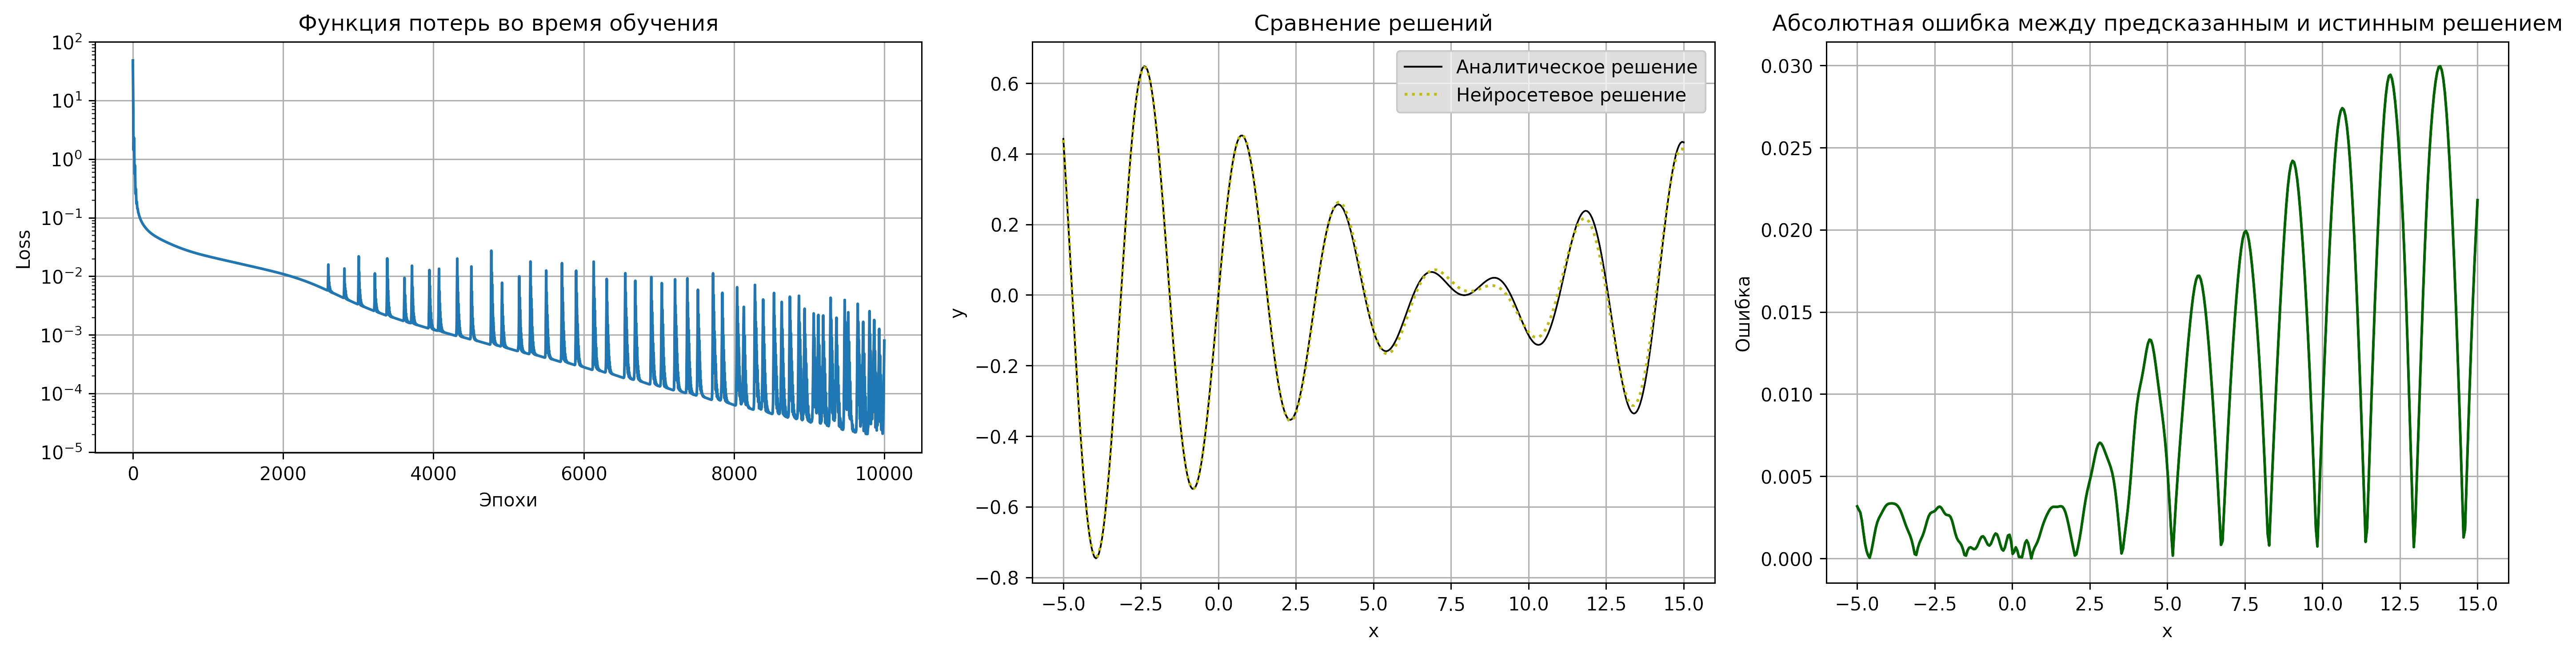
\includegraphics[width=0.8\textwidth]{images/Loss&x_ODE_of_the_first_order_resonance.png}
    \caption{Функция потерь для системы ОДУ первого порядка с резонансом}
    \label{fig:loss_first_order_resonance}
\end{figure}

\begin{table}[h!]
    \centering
    \begin{tabular}{|c|c|c|c|}
    \hline
    \multicolumn{2}{|c|}{\textbf{Без резонанса}} & \multicolumn{2}{|c|}{\textbf{С резонансом}} \\
    \hline
    \textbf{MAE $x, 10^{-2}$} & \textbf{MAE $\dfrac{dx}{dt}, 10^{-2}$} & \textbf{MAE $x, 10^{-2}$} & \textbf{MAE $\dfrac{dx}{dt}, 10^{-2}$} \\
    \hline
    4.8092 & 9.8869 & 0.43286 & 0.8909 \\
    3.5429 & 7.2853 & 0.32455 & 0.6793 \\
    3.6680 & 7.4666 & 0.96157 & 1.9562 \\
    3.6264 & 7.4309 & 0.64427 & 1.3446 \\
    2.5681 & 5.4567 & 0.32558 & 0.6419 \\
    \hline
    \textbf{3.6429} & \textbf{7.5053} & \textbf{0.5378} & \textbf{1.1026} \\
    \hline
    \end{tabular}
    \caption{ОДУ первого порядка}
\end{table}

\begin{itemize}
    \item Более стабильный, но медленный процесс обучения.
    \item Без резонанса среднее MAE больше ОДУ второго порядка в 3 раза.
    \item Лучшая ОДУ для резонанса.
\end{itemize}
\newpage

\subsection{Альтернативная система ОДУ первого порядка (3)}

\begin{figure}[H]
    \centering
    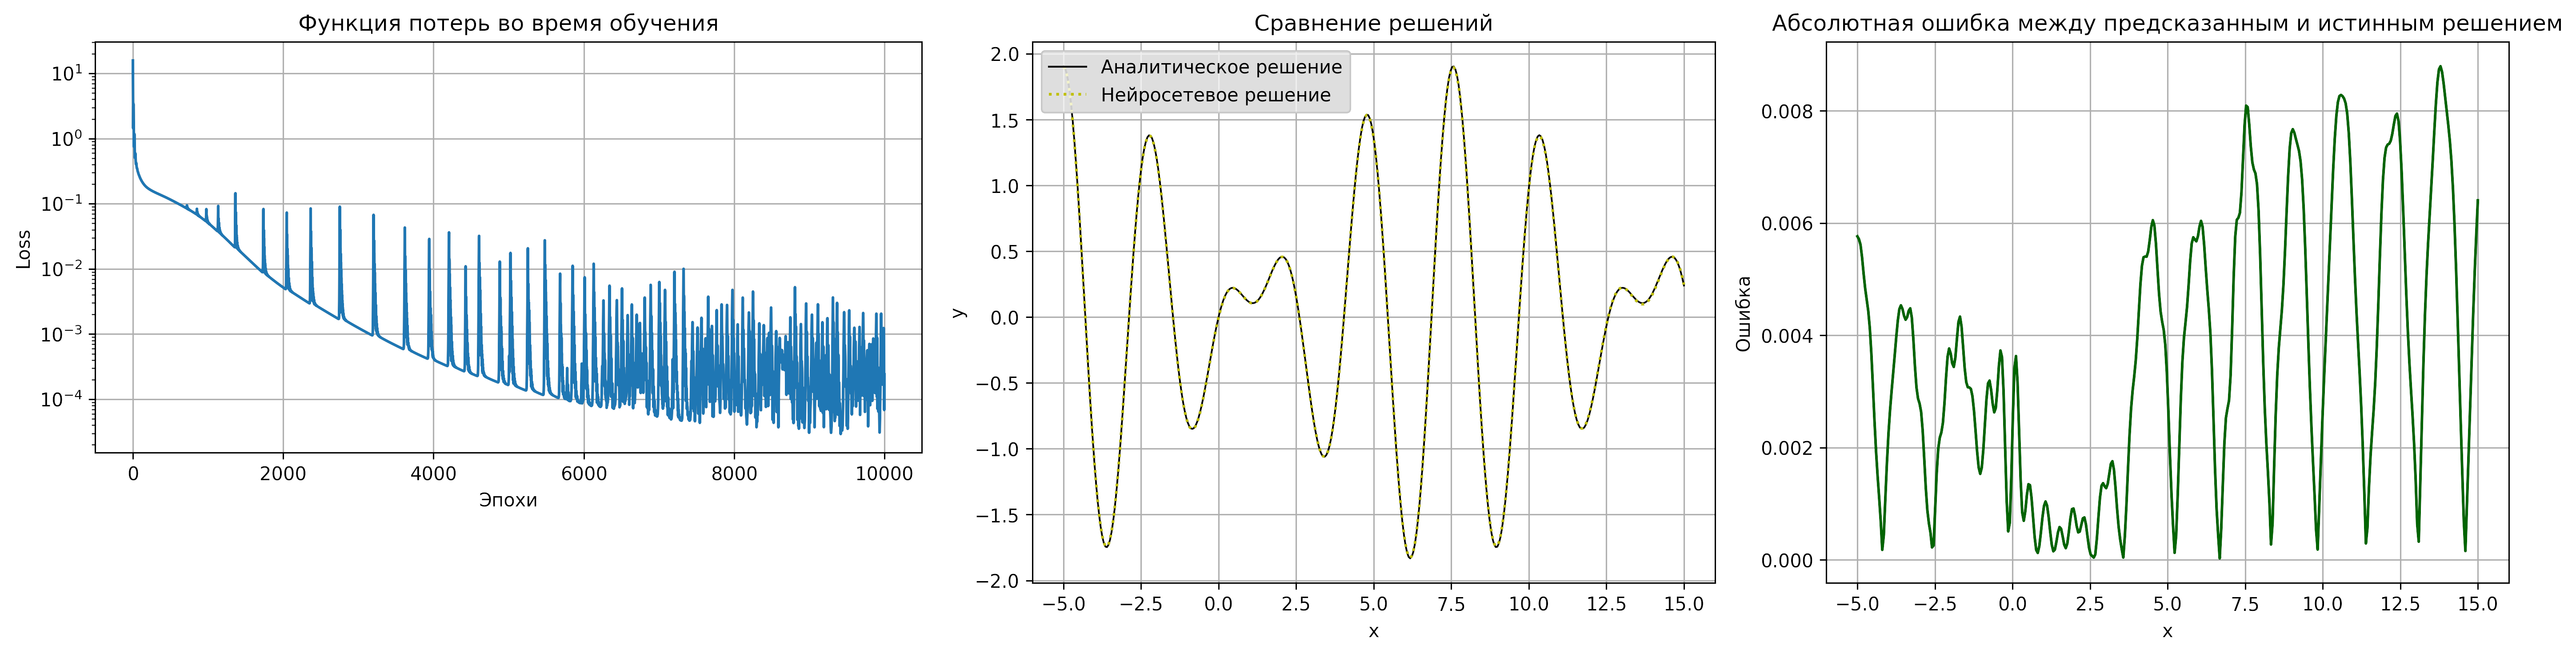
\includegraphics[width=0.8\textwidth]{images/Loss&x_alt_ODE.png}
    \caption{Функция потерь для альтернативной системы ОДУ}
    \label{fig:loss_alt}
\end{figure}

\begin{figure}[H]
    \centering
    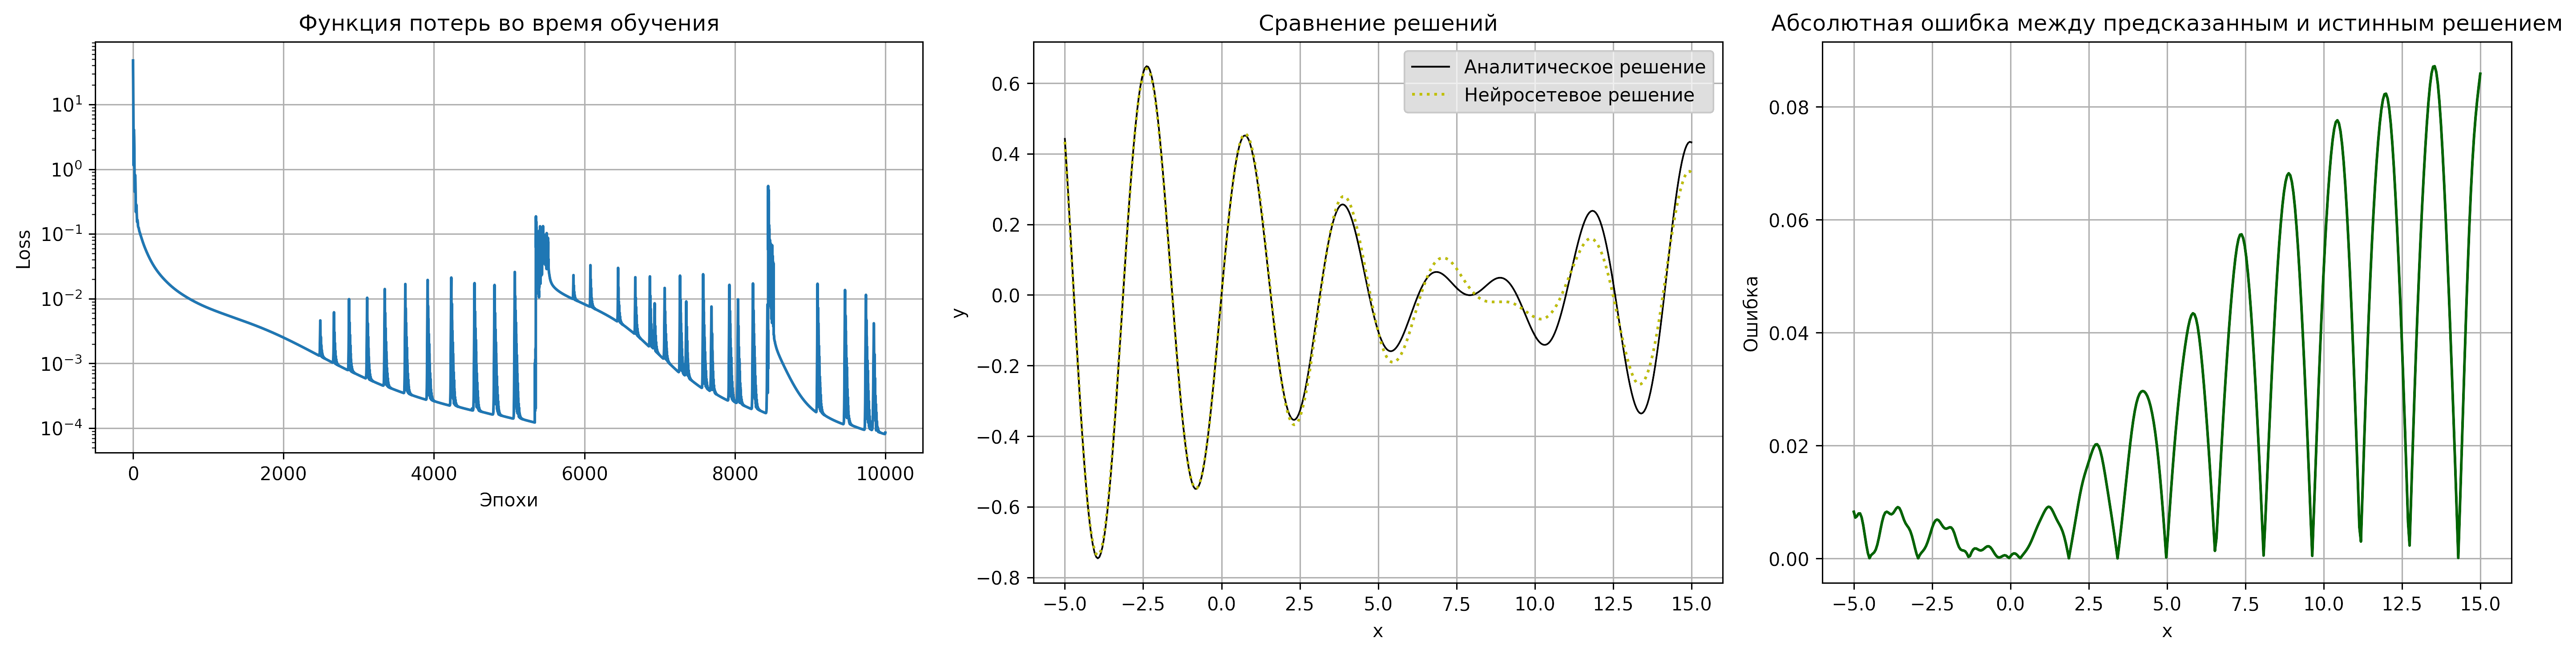
\includegraphics[width=0.8\textwidth]{images/Loss&x_alt_ODE_resonance.png}
    \caption{Функция потерь для альтернативной системы ОДУ с резонансом}
    \label{fig:loss_alt_resonance}
\end{figure}

\begin{table}[h!]
    \centering
    \begin{tabular}{|c|c|c|c|}
    \hline
    \multicolumn{2}{|c|}{\textbf{Без резонанса}} & \multicolumn{2}{|c|}{\textbf{С резонансом}} \\
    \hline
    \textbf{MAE $x, 10^{-2}$} & \textbf{MAE $\dfrac{dx}{dt}, 10^{-2}$} & \textbf{MAE $x, 10^{-2}$} & \textbf{MAE $\dfrac{dx}{dt}, 10^{-2}$} \\
    \hline
    1.0991 & 2,3144 & 1.0198 & 2.2316 \\
    2.4914 & 5,1818 & 0.2385 & 0.5340 \\
    1.0468 & 2,2011 & 1.2542 & 2.6190 \\
    0.4407 & 0,9656 & 1.3087 & 2.7650 \\
    0.9234 & 1,9852 & 0.2077 & 0.4756 \\
    \hline
    \textbf{1.2003} & \textbf{2.5296} & \textbf{0.8058} & \textbf{1.7250} \\
    \hline
    \end{tabular}
    \caption{Альт. ОДУ первого порядка}
\end{table}

\begin{itemize}
    \item Большая точность по сравнению с первой системой.
    \item Менее стабильный процесс обучения.
    \item Достигается точность, близкая к ОДУ второго порядка.
\end{itemize}

\newpage

\subsection{Сравнительный анализ}
\begin{table}[H]
    \centering
    \begin{tabular}{|l|c|c|}
    \hline
    \textbf{Система} & \textbf{Среднее MAE $x$, $10^{-2}$} & \textbf{Среднее MAE $\dfrac{dx}{dt}$, $10^{-2}$} \\
    \hline
    ОДУ второго порядка (1) & 1.1769 & 2.3757 \\
    ОДУ первого порядка (2) & 3.1845 & 7.3041 \\
    Альт. ОДУ первого порядка (3) & 1.3004 & 2.1330 \\
    \hline
    \end{tabular}
    \caption{Сравнительное среднее значение MAE для различных систем без резонанса}
    \label{tab:comparative_mae}
\end{table}

Из таблицы \ref{tab:comparative_mae} видно, что система второго порядка и альтернативная система первого порядка показывают наименьшие значения MAE, что свидетельствует о большей точности и эффективности этих формулировок задачи Коши. Так же хочется заметить, что MAE $x$ приблезительно в 2 раза меньше MAE $\dfrac{dx}{dt}$ во всех экспериментах.

\section{Анализ устойчивости и сходимости}

\subsection{Устойчивость обучения}
Система второго порядка показывает высокую точность, однако часто застревает в локальных минимумах, что снижает устойчивость метода. Система первого порядка (2) демонстрирует более стабильное обучение, но с худшей точностью. Альтернативная система первого порядка (3) сочетает в себе преимущества обеих предыдущих систем, обеспечивая хорошую точность и относительно стабильное обучение.

\subsection{Сходимость метода}
Быстрая сходимость наблюдается для системы второго порядка, что делает её предпочтительной при отсутствии сложных динамических особенностей. Альтернативная система первого порядка показывает сбалансированную скорость сходимости и точность, что может быть полезно в более сложных случаях, таких как системы с резонансом.
\section{Заключение}

Проведённое исследование показывает, что выбор постановки задачи Коши существенно влияет на эффективность и точность метода PINN. Для конкретных приложений имеет смысл сравнить различные формулировки задачи, чтобы подобрать оптимальный вариант. В случае гармонического осциллятора с вынуждающей силой:

\begin{itemize}
    \item \textbf{Использование исходного уравнения второго порядка} даёт быструю сходимость к точному решению, однако могут возникать проблемы с попаданием в локальные минимумы.
    \item \textbf{Преобразование уравнения к системе первого порядка} повышает устойчивость обучения, но может снижать точность и увеличивать время сходимости.
    \item \textbf{Альтернативная система первого порядка} позволяет достичь результата, близкого к исходному уравнению, при этом обладая более стабильным процессом оптимизации.
\end{itemize}

Дополнительно, при наличии резонанса, методы, демонстрирующие лучшую устойчивость и точность, становятся более предпочтительными, так как они способны более точно моделировать сложные динамические поведения системы.

Для дальнейших исследований рекомендуется рассмотреть расширение метода PINN на более сложные системы ОДУ и УЧП, а также исследовать влияние других архитектур нейронных сетей и методов оптимизации на эффективность решения.

Полный код для воспроизведения результатов доступен в репозитории на GitHub:\\
\href{https://github.com/PracticalOscillations/Practice3}{https://github.com/PracticalOscillations/Practice3}.

Мы приглашаем заинтересованных исследователей использовать и развивать представленный подход.

\section{Список литературы}
\begin{thebibliography}{99}
\bibitem{Lagaris1998} Lagaris I.E., Likas A., Fotiadis D.I. Artificial neural networks for solving ordinary and partial differential equations. //IEEE Transactions on Neural Networks, 1998. T. 9. № 5. С. 987–1000.
\bibitem{Raissi2019} Raissi M., Perdikaris P., Karniadakis G.E. Physics-informed neural networks: A deep learning framework for solving forward and inverse problems involving nonlinear partial differential equations. //Journal of Computational Physics, 2019. T. 378. С. 686–707.
\bibitem{PyTorch} \href{https://pytorch.org/docs/stable/index.html}{PyTorch documentation}.
\end{thebibliography}

\end{document}
